\documentclass[a4paper,fleqn]{cas-sc}

\usepackage{graphicx}
\usepackage{url}

\begin{document}

\shorttitle{SAT and Exact Methods for the N-Queens Problem}
\shortauthors{Nguyen Nhat Minh}

\title[mode = title]{A Comparative Study of SAT Encodings and Exact Solvers for the N-Queens Problem}

\author[1]{Nguyen Nhat Minh}[orcid=]
\cormark[1]
\ead{23021631@vnu.edu.vn}

\address[1]{Faculty of Information Technology, VNU University of Engineering and Technology, Vietnam National University, Hanoi, Vietnam}

\cortext[cor1]{Corresponding author.}

\begin{abstract}
The N-Queens problem asks for a placement of $N$ queens on an $N \times N$ chessboard such that no two queens share a row, column, or diagonal. This paper presents a SAT-based solver for the problem and experimentally compares three at-most-one cardinality encodings: pairwise, sequential counter, and bitwise. The SAT approach is evaluated against OR-Tools CP-SAT, CPLEX CP Optimizer, CPLEX MIP, and Gurobi MIP. All methods use a common independent solution validator and a unified benchmark schema recording model size and execution time. Initial local-laptop experiments cover board sizes from $N=8$ to $N=128$. The results show that the relative performance of SAT encodings is strongly size-dependent: pairwise is fastest in the repeated runs through $N=64$, while sequential counter is competitive at smaller sizes and becomes slower as the board grows. CP-SAT and CPLEX CP remain practical in the current extended pilot, whereas restricted CPLEX and Gurobi licenses prevent some larger MIP runs. These results establish a reproducible experimental baseline; final large-instance comparisons will be repeated after academic licenses become available.
\end{abstract}

\begin{highlights}
\item A unified SAT model supports pairwise, sequential-counter, and bitwise AMO encodings.
\item SAT is compared with CP-SAT, CPLEX CP, CPLEX MIP, and Gurobi MIP.
\item All returned solutions are checked by an independent N-Queens validator.
\item Pilot experiments cover board sizes up to $N=128$ on a local laptop.
\item License restrictions are explicitly recorded rather than treated as successful solver runs.
\end{highlights}

\begin{keywords}
N-Queens \sep Boolean satisfiability \sep cardinality encoding \sep constraint programming \sep mixed integer programming \sep exact algorithms
\end{keywords}

\maketitle

\section{Introduction}

The N-Queens problem is a classical constraint satisfaction problem in which $N$ queens must be placed on an $N \times N$ board so that no two queens attack one another. Although the problem has a simple statement, it is a useful benchmark for comparing exact solving paradigms because the number of possible placements grows rapidly with $N$ and the constraints can be represented using several modelling formalisms.

This study focuses on a SAT formulation and compares it with exact methods based on constraint programming and mixed integer programming. The SAT part is implemented with PySAT and the Glucose3 solver~\citep{ignatiev2018pysat}. Three at-most-one (AMO) encodings are evaluated while the underlying SAT solver and N-Queens constraints remain fixed. This design isolates the effect of the cardinality encoding~\citep{sinz2005cardinality}.

The contributions of this work are:
\begin{itemize}
    \item a reusable SAT encoding architecture for N-Queens;
    \item an implementation of pairwise, sequential-counter, and bitwise AMO encodings;
    \item implementations of CP-SAT, CPLEX CP, CPLEX MIP, and Gurobi MIP models;
    \item a common validator and benchmark result schema;
    \item a pilot comparison of model size, execution time, solver status, and license limitations.
\end{itemize}

\section{Problem Definition and Mathematical Models}

Let $x_{r,c}$ denote whether a queen is placed at row $r$ and column $c$, where $0 \le r,c < N$. The N-Queens constraints require exactly one queen in each row and column and at most one queen on each diagonal.

For SAT and MIP, $x_{r,c}$ is a Boolean or binary decision variable. The row constraints are:
\begin{equation}
\sum_{c=0}^{N-1} x_{r,c} = 1 \qquad \forall r.
\end{equation}
The column constraints are:
\begin{equation}
\sum_{r=0}^{N-1} x_{r,c} = 1 \qquad \forall c.
\end{equation}
For each main diagonal and anti-diagonal, the corresponding variables satisfy an at-most-one constraint. Main diagonals are grouped by $r-c$ and anti-diagonals by $r+c$.

The CP and CP-SAT models use $N$ integer variables $q_r$, where $q_r$ is the column assigned to row $r$. They enforce:
\begin{equation}
\operatorname{AllDifferent}(q_r),\quad
\operatorname{AllDifferent}(q_r+r),\quad
\operatorname{AllDifferent}(q_r-r).
\end{equation}

\section{SAT-Based Approach}

\subsection{CNF Encoding}

Each board position is mapped to a SAT variable using:
\begin{equation}
v(r,c) = rN+c+1.
\end{equation}
Exactly-one constraints are decomposed into an at-least-one clause and an AMO constraint. The implementation uses a shared PySAT \texttt{IDPool} whose auxiliary variables start after the $N^2$ original board variables. This prevents auxiliary-variable collisions across rows, columns, and diagonals.

\subsection{AMO Encodings}

The pairwise encoding adds one binary clause $\lnot x_i \lor \lnot x_j$ for every pair of literals. It introduces no auxiliary variables but can produce a quadratic number of clauses.

The sequential-counter encoding introduces auxiliary variables representing partial prefix counts. It generally provides a more compact clause structure than pairwise encoding for larger cardinality constraints, at the cost of additional variables.

The bitwise encoding introduces binary selector variables. It provides another trade-off between the number of auxiliary variables and clauses. All three encodings are supplied with the same N-Queens constraints and solved by Glucose3.

\subsection{Solution Decoding and Validation}

If the SAT instance is satisfiable, the model is decoded into the representation $q_r=c$. The decoded placement is then checked independently. The validator verifies the board size, column bounds, column uniqueness, main-diagonal uniqueness, and anti-diagonal uniqueness. This validation is separate from the solver model implementation.

\section{Compared Exact Solvers}

The study compares the SAT solver with four exact alternatives. OR-Tools CP-SAT~\citep{ortools} uses the integer-variable formulation and records conflicts and branches where available. CPLEX CP Optimizer~\citep{cplex} uses the same high-level all-different formulation. CPLEX MIP and Gurobi MIP~\citep{gurobi} use binary board-position variables and linear row, column, and diagonal constraints.

The benchmark runner normalizes all solver outputs into a common schema containing status, validity, model-size fields where available, build or encoding time, solve time, total time, raw status, and error information.

\section{Experimental Setup}

\subsection{Hardware and Software}

Experiments were executed on a local laptop using Python 3.11. The environment was verified for PySAT with Glucose3, OR-Tools, Gurobi, CPLEX MIP, and CPLEX CP Optimizer. The automated test suite contains 43 passing tests.

\subsection{Benchmark Protocol}

The SAT encoding experiment uses $N=8,16,32,64,96,128$. The completed repeated local batch uses five repeats for $N \le 32$ and three repeats for $N=64$. Earlier pilot data covers $N=96$ and $N=128$ with one run per encoding.

The cross-solver core experiment uses $N=8,16,24,31,32$. The extended experiment uses $N=44,45,64,100,128$ with one run per solver. The hard timeout is 600 seconds per solver configuration. A solver that exceeds the timeout is recorded as \texttt{TIMEOUT}; a solver rejected by its license is recorded as \texttt{LICENSE\_LIMIT}. Neither status stops the remaining configurations.

\subsection{Reproducibility}

Source code, benchmark outputs, summary tables, and figures are maintained in the project repository:
\begin{quote}
\url{https://github.com/nNm205/n-queens-solving}
\end{quote}

\section{Experimental Results}

\subsection{SAT Encoding Comparison}

Table~\ref{tab:sat-summary} reports median total times from the repeated local batch. Pairwise is the fastest encoding at all four sizes in this batch. Sequential counter is competitive at $N=16$, while bitwise becomes substantially slower at $N=32$ and $N=64$ in these runs.

\begin{table}[width=.95\linewidth,cols=4,pos=ht]
\caption{Median total time in seconds for the repeated SAT encoding batch.}
\label{tab:sat-summary}
\begin{tabular}{lrrrr}
\hline
$N$ & Pairwise & Sequential counter & Bitwise & Repeats \\
\hline
8  & 0.0010 & 0.0015 & 0.0013 & 5 \\
16 & 0.0158 & 0.0086 & 0.1042 & 5 \\
32 & 0.0749 & 0.4728 & 15.7860 & 5 \\
64 & 0.6018 & 10.2342 & 6.2919 & 3 \\
\hline
\end{tabular}
\end{table}

The earlier pilot results at $N=96$ and $N=128$ show that runtime is not monotonic for every encoding. In particular, the observed bitwise runtime varies considerably between runs and board sizes. Therefore, the final cross-solver baseline should be selected after considering repeated measurements, clause counts, and runtime stability rather than one isolated large-instance result.

\subsection{Cross-Solver Comparison}

Table~\ref{tab:solver-summary} gives selected results from the core and extended experiments. CP-SAT and CPLEX CP remain practical through $N=128$ in the current local environment. Gurobi solves the $N=32$ case but is blocked by its restricted license in larger tested cases. CPLEX MIP is blocked at $N=32$ and above by the Community Edition model-size restriction.

\begin{table}[width=.98\linewidth,cols=6,pos=ht]
\caption{Selected cross-solver results from the current local phase. Times are total seconds; a dash denotes a license-limited run.}
\label{tab:solver-summary}
\begin{tabular}{lrrrrr}
\hline
$N$ & SAT & CP-SAT & CPLEX CP & CPLEX MIP & Gurobi MIP \\
\hline
8   & 0.004 & 0.036 & 0.054 & 0.036 & 0.005 \\
16  & 0.249 & 0.076 & 0.054 & 0.045 & 0.045 \\
24  & 16.571 & 0.120 & 0.056 & 0.057 & 0.014 \\
31  & 9.598 & 0.197 & 0.060 & 0.073 & 0.077 \\
32  & 51.042 & 0.200 & 0.059 & -- & 0.081 \\
44  & 266.893 & 0.360 & 0.062 & -- & 0.164 \\
64  & 21.493 & 0.837 & 0.067 & -- & -- \\
128 & 3.231 & 4.448 & 0.078 & -- & -- \\
\hline
\end{tabular}
\end{table}

The cross-solver SAT column uses the bitwise candidate baseline and only one run per configuration. Its non-monotonic runtime pattern should therefore be interpreted cautiously. The results are suitable for a pilot comparison, but final statistical claims require repeated runs under the same license conditions.

\begin{figure}[width=.95\linewidth,pos=ht]
\centering
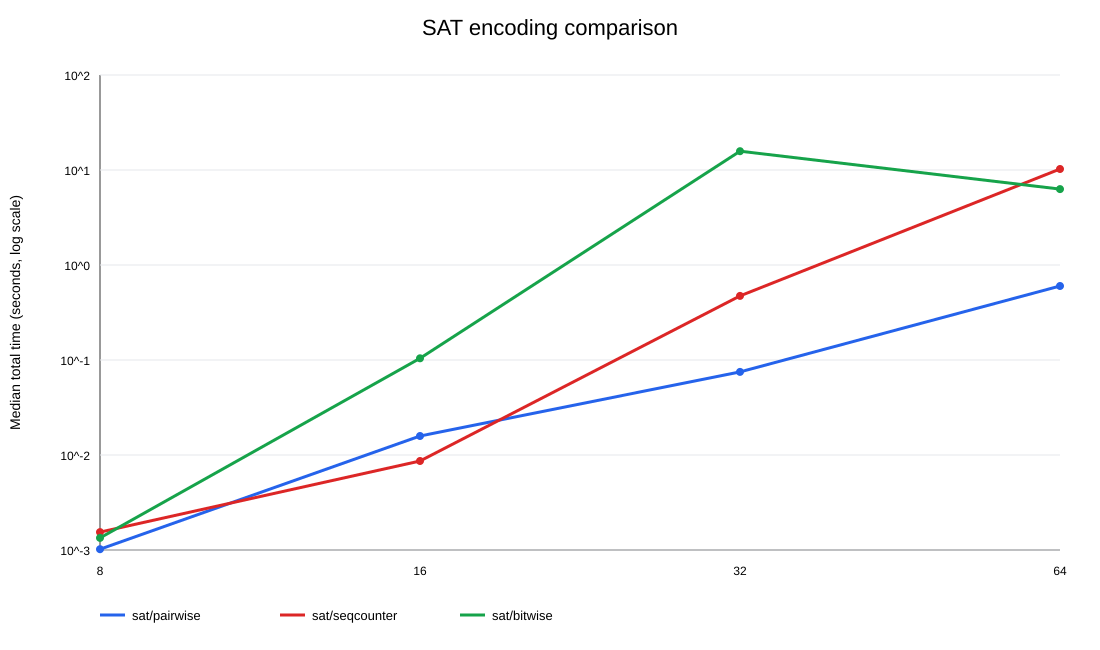
\includegraphics[width=\linewidth]{sat_encoding_runtime.svg}
\caption{SAT encoding runtime comparison from the repeated local batch.}
\label{fig:sat-runtime}
\end{figure}

\begin{figure}[width=.95\linewidth,pos=ht]
\centering
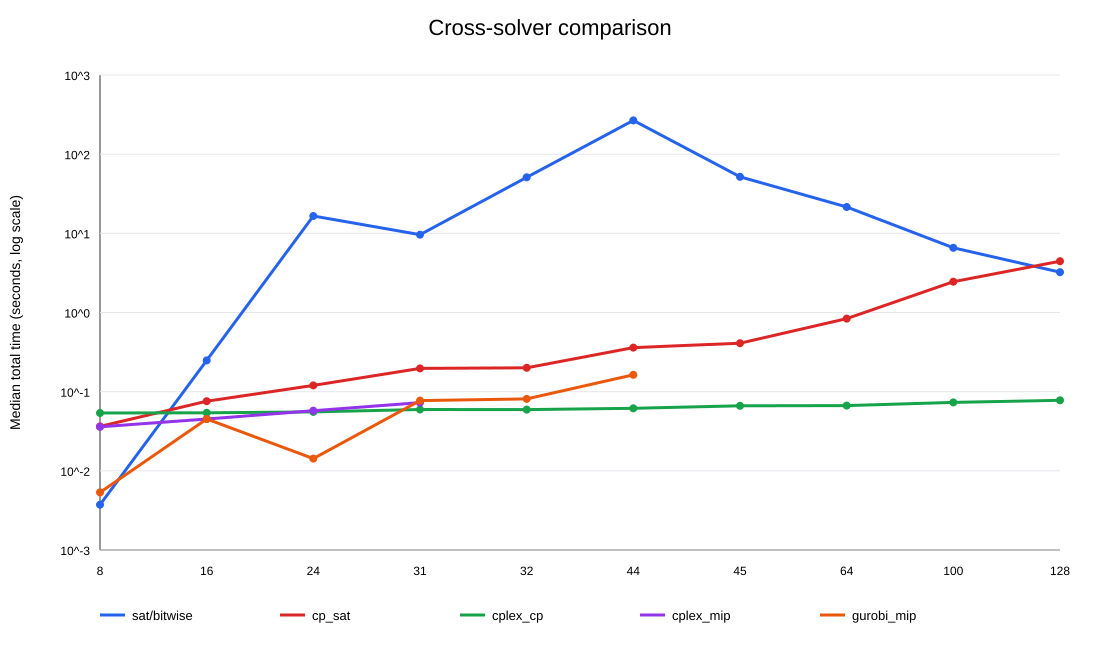
\includegraphics[width=\linewidth]{solver_runtime.svg}
\caption{Cross-solver runtime comparison on a logarithmic scale.}
\label{fig:solver-runtime}
\end{figure}

\section{Limitations and Discussion}

The current experiments are limited by restricted solver licenses. CPLEX Community Edition rejects the $N=32$ MIP model because it contains 1024 binary variables. Gurobi's restricted license rejects some larger models, including the tested $N=45$ and above cases. These outcomes are reported explicitly and are not interpreted as solver failures caused by the mathematical formulation.

The repeated SAT encoding experiment and the one-run cross-solver experiment also have different statistical strength. The former supports a preliminary comparison of median runtime, while the latter is primarily a feasibility and scalability pilot. After academic licenses are activated, the core and extended cross-solver experiments should be repeated and the tables in this section should be regenerated.

\section{Conclusion}

This paper presented a unified implementation for solving N-Queens with SAT, constraint programming, and mixed integer programming. The SAT implementation supports three AMO encodings and includes independent solution validation. The benchmark infrastructure records common performance and status fields and continues after solver-specific errors.

The current local results show that no single AMO encoding dominates across all tested sizes. Pairwise performs best in the repeated batch through $N=64$, sequential counter is competitive at smaller sizes, and bitwise exhibits substantial runtime variation. CP-SAT and CPLEX CP provide stable results in the extended pilot, while the MIP comparison remains incomplete until unrestricted licenses are available. The next step is to repeat the large cross-solver experiments after license activation and use the resulting data for the final report tables and conclusions.

\printcredits

\section*{Declaration of Competing Interest}
The author declares that there is no known competing financial interest or personal relationship that could have appeared to influence the work reported in this paper.

\section*{Data Availability}
Source code, benchmark result files, summary tables, and figures are available at:
\url{https://github.com/nNm205/n-queens-solving}

\section*{Declaration of Generative AI and AI-Assisted Technologies}
During the preparation of this work, the author used ChatGPT by OpenAI to assist with language revision, code organization, and analysis drafting. The author reviewed and edited the generated material and takes full responsibility for the final content.

\bibliographystyle{cas-model2-names}
\bibliography{references}

\end{document}
